\begin{figure}[h!]
	\centering
	
	
	
	\tikzset{every picture/.style={line width=0.75pt}} %set default line width to 0.75pt        
	
	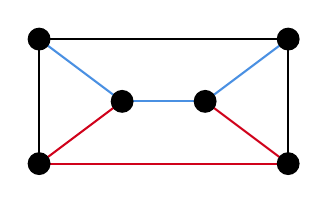
\begin{tikzpicture}[x=0.75pt,y=0.75pt,yscale=-1,xscale=1]
		%uncomment if require: \path (0,300); %set diagram left start at 0, and has height of 300
		
		%Straight Lines [id:da29435505087653746] 
		\draw [color={rgb, 255:red, 208; green, 2; blue, 27 }  ,draw opacity=1 ][fill={rgb, 255:red, 74; green, 144; blue, 226 }  ,fill opacity=1 ]   (195,105) -- (235,75) ;
		%Straight Lines [id:da15130033487443384] 
		\draw [color={rgb, 255:red, 208; green, 2; blue, 27 }  ,draw opacity=1 ][fill={rgb, 255:red, 74; green, 144; blue, 226 }  ,fill opacity=1 ]   (195,105) -- (315,105) ;
		%Straight Lines [id:da9313777412496024] 
		\draw [color={rgb, 255:red, 208; green, 2; blue, 27 }  ,draw opacity=1 ][fill={rgb, 255:red, 74; green, 144; blue, 226 }  ,fill opacity=1 ]   (275,75) -- (315,105) ;
		%Straight Lines [id:da979754963449776] 
		\draw [color={rgb, 255:red, 74; green, 144; blue, 226 }  ,draw opacity=1 ][fill={rgb, 255:red, 74; green, 144; blue, 226 }  ,fill opacity=1 ]   (275,75) -- (235,75) ;
		%Straight Lines [id:da11218419538778379] 
		\draw [color={rgb, 255:red, 74; green, 144; blue, 226 }  ,draw opacity=1 ][fill={rgb, 255:red, 74; green, 144; blue, 226 }  ,fill opacity=1 ]   (315,45) -- (275,75) ;
		%Straight Lines [id:da44553444033080924] 
		\draw [color={rgb, 255:red, 74; green, 144; blue, 226 }  ,draw opacity=1 ][fill={rgb, 255:red, 74; green, 144; blue, 226 }  ,fill opacity=1 ]   (235,75) -- (195,45) ;
		%Shape: Circle [id:dp5069495015265886] 
		\draw  [fill={rgb, 255:red, 0; green, 0; blue, 0 }  ,fill opacity=1 ] (190,45) .. controls (190,42.24) and (192.24,40) .. (195,40) .. controls (197.76,40) and (200,42.24) .. (200,45) .. controls (200,47.76) and (197.76,50) .. (195,50) .. controls (192.24,50) and (190,47.76) .. (190,45) -- cycle ;
		%Shape: Circle [id:dp25021666713761814] 
		\draw  [fill={rgb, 255:red, 0; green, 0; blue, 0 }  ,fill opacity=1 ] (190,105) .. controls (190,102.24) and (192.24,100) .. (195,100) .. controls (197.76,100) and (200,102.24) .. (200,105) .. controls (200,107.76) and (197.76,110) .. (195,110) .. controls (192.24,110) and (190,107.76) .. (190,105) -- cycle ;
		%Shape: Circle [id:dp606959925111063] 
		\draw  [fill={rgb, 255:red, 0; green, 0; blue, 0 }  ,fill opacity=1 ] (310,45) .. controls (310,42.24) and (312.24,40) .. (315,40) .. controls (317.76,40) and (320,42.24) .. (320,45) .. controls (320,47.76) and (317.76,50) .. (315,50) .. controls (312.24,50) and (310,47.76) .. (310,45) -- cycle ;
		%Shape: Circle [id:dp7417260861337834] 
		\draw  [fill={rgb, 255:red, 0; green, 0; blue, 0 }  ,fill opacity=1 ] (310,105) .. controls (310,102.24) and (312.24,100) .. (315,100) .. controls (317.76,100) and (320,102.24) .. (320,105) .. controls (320,107.76) and (317.76,110) .. (315,110) .. controls (312.24,110) and (310,107.76) .. (310,105) -- cycle ;
		%Shape: Circle [id:dp47320961285111385] 
		\draw  [fill={rgb, 255:red, 0; green, 0; blue, 0 }  ,fill opacity=1 ] (230,75) .. controls (230,72.24) and (232.24,70) .. (235,70) .. controls (237.76,70) and (240,72.24) .. (240,75) .. controls (240,77.76) and (237.76,80) .. (235,80) .. controls (232.24,80) and (230,77.76) .. (230,75) -- cycle ;
		%Shape: Circle [id:dp9913663913060298] 
		\draw  [fill={rgb, 255:red, 0; green, 0; blue, 0 }  ,fill opacity=1 ] (270,75) .. controls (270,72.24) and (272.24,70) .. (275,70) .. controls (277.76,70) and (280,72.24) .. (280,75) .. controls (280,77.76) and (277.76,80) .. (275,80) .. controls (272.24,80) and (270,77.76) .. (270,75) -- cycle ;
		%Straight Lines [id:da7053823784402796] 
		\draw    (195,45) -- (315,45) ;
		%Straight Lines [id:da848171725259851] 
		\draw    (315,45) -- (315,105) ;
		%Straight Lines [id:da2625430487899586] 
		\draw    (195,105) -- (195,45) ;
		
		
		
		
	\end{tikzpicture}
\end{figure}